\documentclass[a4paper,utf8]{article}
\usepackage[heading,fancyhdr]{ctex}
\usepackage{amsmath,amssymb,geometry,lastpage,ulem}
\usepackage{array,tabularx,graphicx}
\geometry{
    top=25.4mm, 
    left=30mm, 
    right=30mm, 
    bottom=35mm,
    headsep=5.9mm,
}
\ctexset{
    section = {format+=\raggedright}
}
\newcommand{\expinfo}[5]{
    {\zihao{-3}\bfseries\songti
    实验名称:\uline{\hfill\mbox{#1}\hfill} \\[2.9mm]
    学\quad 号:\uline{\makebox[25mm]{#2}}\hfill
    姓\quad 名:\uline{\makebox[25mm]{#3}}\hfill
    班\quad 级:\uline{\makebox[25mm]{#4}} \\[2.9mm]
    合作者:\uline{\makebox[25mm]{无}}\enspace~
    桌\quad号:\uline{\makebox[25mm]{}}\hfill\mbox{}\\[2.9mm]
    指导教师:\uline{\makebox[30mm]{#5}}\hfill\mbox{} \\[2.9mm]
    实验日期:\uline{\makebox[30mm]{}}\hfill\mbox{} \\[58.7mm]
    }
}%\expinfo{实验名称}{学号}{姓名}{班级}{指导教师}
\pagestyle{fancy}
\fancyhf{} \fancyhead[C]{材料科学基础实验} \fancyfoot[C]{\thepage~/~\pageref{LastPage}}
\begin{document}
\begin{center}
    {\mbox{}\\[7em]\zihao{2}\bfseries\songti%
    材料科学基础实验报告}\\[34mm]
    \expinfo{实验一 铁碳合金的显微组织观察及性能分析}{22301070}{杨雨燃}{22材物}{杨玉华}
\end{center}
\newpage
\section*{【实验目的】}
    \begin{enumerate}
        \item 了解金相显微镜的成像基本原理、构造、主要部件及作用;
        \item 熟悉金相显微镜的使用和其注意事项;
        \item 掌握分析铁碳合金在平衡状态下及不同工艺热处理后的显微组织形态;
        \item 加深理解铁碳合金组织与性能之间的关系。
    \end{enumerate}   
\section*{【实验原理】}%简单描述,含必要的公式和附图;
    \begin{enumerate}
        \item 金相分析是研究材料内部组织和缺陷的主要方法之一,是研究金属材料微观结构最基本的一种实验技术。通过显微分析可以研究材料内部的组织与其化学成分的关系;确定各类材料经不同方式加工及热处理后的显微组织;判断材料质量的优劣,如金属材料中诸如氧化物、硫化物等各种非金属夹杂物在显微组织中的大小、数量、分布情况以及晶粒度的大小等。
        \item 金相显微镜的成像原理如图:
        
        \begin{center}
            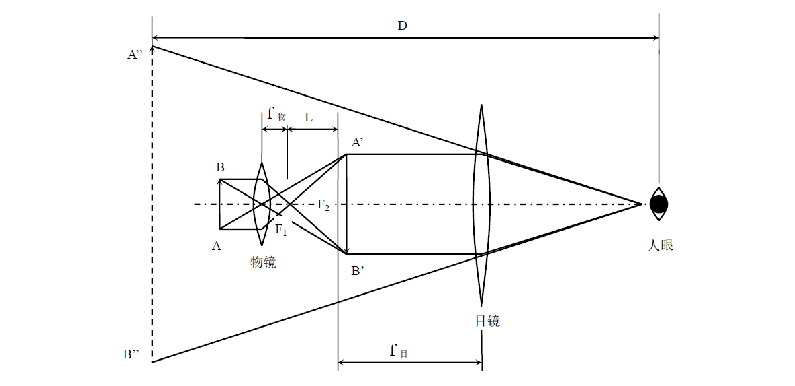
\includegraphics[width=300pt]{1.png}
        \end{center}
        
        显微镜的放大倍数为:
                       $M = M_\text{物} * M_\text{目}$
        \item 金相显微镜的主要性能参数:
        \item 
        ①物镜的数值孔径
        
        ②分辨率(横向分辨率)

        ③焦深(垂直分辨率)
        \item 金相显微镜的构造:
        \begin{center}
            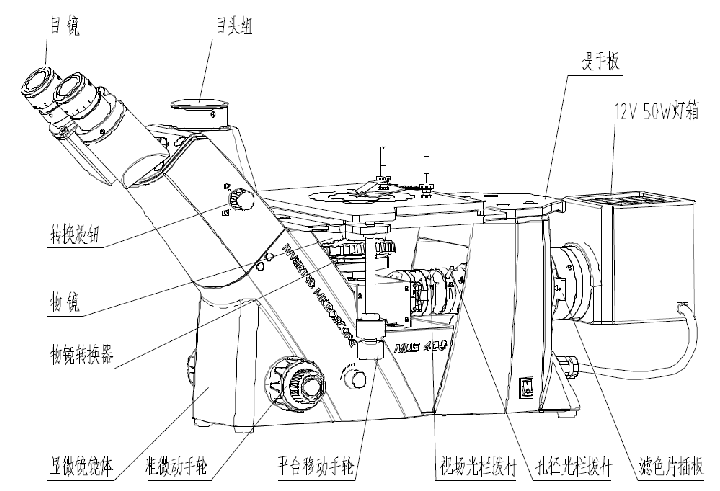
\includegraphics[width=400pt]{2.png} 
        \end{center}
        \item 七种典型铁碳合金:

    ①工业纯铁:含碳量小于0.0218\%,室温下显微组织由白色块状铁素体和极少量三次渗碳体(通常可忽略)构成。用硝酸酒精浸蚀后显微组织呈白色多边形,晶界呈黑色网状

    ②亚共析钢:含碳量为0.0218\%~0.77\%,在显微镜下观察时,若珠光体的层片间距较大或者放大倍数较高时其呈片层状,且可清楚地看到珠光体中平行相间的宽条铁素体和细条渗碳体;若珠光体在层片间距较小或者放大倍数较低时,则其片层结构不能分辨,呈暗黑色。另随着含碳量的增加,珠光体含量增加,铁素体含量减少。
    
    ③共析钢:含碳量为0.77\%,室温下的显微组织全部由层片状珠光体(P)组织构成,即片状铁素体和渗碳体的机械混合物,且铁素体与渗碳体质量比约为7.9:1,铁素体厚,渗碳体薄。用硝酸酒精浸蚀后,珠光体中铁素体与渗碳体都呈白亮色,只有相界呈黑色。
    
    ④过共析钢:含碳量为0.77\%~2.11\%,室温下的显微组织由白亮色网状二次渗碳体和层片状珠光体(P)构成。用硝酸酒精浸蚀后,二次渗碳体成亮白色网分布在珠光体的周围。
    
    ⑤亚共晶白口铸铁:含碳量为2.11\%~4.3\%,室温下的显微组织由黑色树枝状珠光体(P)、二次渗碳体和豹皮状低温莱氏体构成,二次渗碳体在珠光体周围析出,与莱氏体中的渗碳体连在一起,难以分辨。
    
    ⑥共晶白口铸铁:含碳量为4.3\%,室温下的显微组织由豹皮状低温莱氏体构成,其中白色集体为共晶渗碳体,黑色粒状或棒状组织为珠光体,其片层状无法分辨而成黑色。
    
    ⑦过共晶白口铸铁:含碳量为4.3\%~6.69\%,室温下的显微组织由一次渗碳体和低温莱氏体构成,其中的一次渗碳体呈白亮色板条状分布在低温莱氏体中。
    \end{enumerate}



\section*{【实验仪器】}%规格及参数
1、MDS400倒置式金相显微镜

2、铁碳合金平衡状态金相试样×1,多种热处理方式之后的碳钢式样×1
\section*{【实验过程】}%简述主要过程和实验内容

1. 领取一套经不同热处理工艺的45钢及T12钢标准试样(21\#-27\#),在显微镜下观察经
不同热处理工艺的45钢及T12试样。理解并分析不同热处理工艺条件下试样的组织变化,认
真体会整个操作过程,并将观察图像拍照存储。
其中:
21\#为45钢860℃水淬+中温回火;
22\#为45钢860℃水淬+高温回火;
23\#为45钢780℃水淬;
24\#为45钢1100℃水淬;
25\#为T12钢球化退火;
26\#为T12钢780℃水淬+低温回火;
27\#为T12钢1100℃水淬+低温回火。

2.注意事项:
1、操作时必须特别谨慎,不能有任何剧烈的动作,不允许自行拆卸光学系统。

2、在旋转粗调或微调旋钮时动作要慢,碰到某种障碍时应立即停止操作,报告指导教师查找
原因,不得用力强行转动,否则会损坏机件。

3、要爱护已制备好的金相试样。不能用手触摸试样的观察面,如有尘埃等脏物不能用嘴吹,
也不能随意擦,要用吸耳球吹除或用无水酒精冲洗并干燥。

4、试样观察完毕后要放入干燥箱中保存。

\section*{【实验数据】}
手绘图:

图片数据,按编号如下:




\end{document}